\documentclass[a4paper,11pt]{article}



% \sffamily %schrift ohne Serifen

\usepackage[T1]{fontenc} 
% schriftencodierung f�r umlaute, trennung
% f\"ur Uni
\usepackage[ansinew]{inputenc}
\usepackage{selinput}
% \usepackage[utf8]{inputenc} 
\usepackage{bibgerm} 
% german bibliography
\usepackage[german]{babel}
%wichtig f�r deutschen Content
\usepackage{ucs}
%erweiterte UTF-8 Unterst�tzung
\usepackage{wrapfig} 
% Paket zur Positionierung einbinden
\usepackage{multirow}
% zusammenfassen von Tabellenzellen
% \usepackage{subscript}
% zum tiefstellen
\usepackage{lscape}
\usepackage{pdflscape}
% zum drehen der Seite
% \usepackage[super]{natbib}
\usepackage[square,sort,comma,numbers]{natbib}
% Erstellung es Literaturverzeichnisses
\usepackage{url}
% Umbruch f�r URL
\usepackage{pst-3dplot}
% f�r tex Grafiken n�tig
\usepackage{pstricks}
\usepackage{listings}
% f�r das einf�gen von Quelltext
\definecolor{codegray}{rgb}{0.92,0.92,0.92}
\lstset{basicstyle=\fontsize{9}{11}\selectfont\ttfamily, breaklines=true, backgroundcolor=\color{codegray}, numbers=left, numberstyle=\tiny, tabsize=4, language=java}
\definecolor{mymauve}{rgb}{0.58,0,0.82}
\definecolor{mygreen}{rgb}{0,0.6,0}
\lstset{
commentstyle=\color{mygreen},
keywordstyle=\color{mymauve},
language=Java,
stringstyle=\color{blue}
}


%Einstellungen f�r Quellcode
\usepackage[a4paper, left=3cm, right=2cm, top=2cm]{geometry}
% Formatierung R�nder
\usepackage[section]{placeins}
% f�r Floatbarriere
\usepackage{color}
%f�r die Verwendung von Farben

\clubpenalty = 10000 
\widowpenalty = 10000
\displaywidowpenalty = 10000
%Verhinderung von Hurenkindern und Schusterjungen
%10000 bedeutet die sie sollen kommplett vermieden werden

\title{Serialisierung von Datenobjekten in JSON zur \"Ubertragung von Objekten aus Energieanwendungen}

\author{Sebastian Rieger}

\pagenumbering{arabic}
%Seitenzahlen(arabische Zahlen)

\setlength{\parindent}{0.25cm} 
%Absatzeinzug �ndern in Zoll
\setlength{\parskip}{0.25cm}
%Absatzabstand
\linespread {1.5}
%Zeilenabstand

% \usepackage{hyperref}
%anklickbare Hyperlinks

%funktioniert nicht bei Fu�noten
\usepackage{graphicx}
\usepackage{graphics}
%f�r einbinden von Grafiken
\usepackage{setspace}
\usepackage{framed}
%f�r Umrandung der Erkl�rung
\usepackage{acronym}
% f�r abk�rzungen
% \usepackage{PSTricks}
\usepackage{epstopdf}
% f�r eps bilder nutze pdflatex --shell-escape this.tex
\usepackage{amssymb}
% f�r mathematische Symbole

\usepackage{hyperref}
% klickbare links

% \usepackage{pdfpages}
\usepackage{rotating}
%%%%%%%%%%%%%%%%%%%%%%%%%%%%%%%%%%%%%%%%%%%%%%%%%%%%%%%%%%%%%%%%%%%%%%%%%%%%%%%%%%%%%%%%%%%%%%%%%%%%%
%% Angaben zur Arbeit
%%%%%%%%%%%%%%%%%%%%%%%%%%%%%%%%%%%%%%%%%%%%%%%%%%%%%%%%%%%%%%%%%%%%%%%%%%%%%%%

\newcommand{\Autor}{Sebastian Rieger}
\newcommand{\MatrikelNummer}{7406886}
\newcommand{\Kursbezeichnung}{TINF12B1}

\newcommand{\FirmenName}{Karlsruher Institut f�r Technologie (KIT)}
\newcommand{\FirmenStadt}{Karlsruhe}
\newcommand{\FirmenLogoDeckblatt}{{
\includegraphics[width=3cm]{Bilder/kitlogo}}}

% Falls es kein Firmenlogo gibt:
%  \newcommand{\FirmenLogoDeckblatt}{}

\newcommand{\BetreuerFirma}{Dr.-Ing. Karl-Uwe Stucky}
% \newcommand{\BetreuerDHBW}{Titel Vorname Nachname}
\newcommand{\Titel}{Serialisierung von Datenobjekten in JSON zur \"Ubertragung von Objekten aus Energieanwendungen}
\newcommand{\AbgabeDatum}{15. September 2014}

\newcommand{\Dauer}{13 Wochen}

% \newcommand{\Abschluss}{Bachelor of Engineering}
\newcommand{\Abschluss}{Bachelor of Science}

\newcommand{\Studiengang}{Angewandte Informatik}
% \newcommand{\Studiengang}{Angewandte Informatik}
\newcommand{\Was}{Projektarbeit}

%%%%%%%%%%%%%%%%%%%%%%%%%%%%%%%%%%%%%%%%%%%%%%%%%%%%%%%%%%%%%%%%%%%%%%%%%%%%%%%%%%%%%%%%%%%%%%%%%%%%% 
%steuervariable
\usepackage{ifthen} %Package f�r if/else
\newboolean{bilder} %Deklaration
\setboolean{bilder}{true} %Zuweisung
% \setboolean{bilder}{false} %Zuweisung
%%%%%%%%%%%%%%%%%%%%%%%%%%%%%%%%%%%%%%%%%%%%%%%%%%%%%%%%%%%%%%%%%%%%%%%%%%%%%%%%%%%%%%%%%%%%%%%%%%%%%

\begin{document}

\begin{center}
\vspace*{-2cm}
\FirmenLogoDeckblatt\hfill
\includegraphics[width=4cm]{Bilder/dhbw-logo}\\[1cm]
{\Huge \Titel}\\[2cm]
{\Huge\scshape \Was}\\[2cm]
{\large f�r die Pr�fung zum}\\[0.5cm]
{\Large \Abschluss}\\[0.5cm]
{\large des Studienganges \Studiengang}\\[0.5cm]
{\large an der}\\[0.5cm]
{\large Dualen Hochschule Baden-W�rttemberg Karlsruhe}\\[0.5cm]
{\large von}\\[0.5cm]
{\large\bfseries \Autor}\\[1cm]
{\large Abgabedatum \AbgabeDatum}
\vfill
\end{center}
\begin{tabular}{l@{\hspace{1cm}}l}
Bearbeitungszeitraum             & \Dauer                       \\
Matrikelnummer                   & \MatrikelNummer              \\
Kurs                             & \Kursbezeichnung             \\
Ausbildungsfirma                 & \FirmenName                  \\
                                 & \FirmenStadt                 \\
Betreuer der Ausbildungsfirma    & \BetreuerFirma               \\
% Gutachter der Studienakademie    & \BetreuerDHBW                \\
\end{tabular}

\newpage
%Seitenumbruch
%%%%%%%%%%%%%%%%%%%%%%%%%%%%%%%%%%%%%%%%%%%%%%%%%%%%%%%%%%%%%%%%%%%%%%%%%%%%%%
%% Descr:       Vorlage für Berichte der DHBW-Karlsruhe, Erklärung
%% Author:      Prof. Dr. Jürgen Vollmer, vollmer@dhbw-karlsruhe.de
%% $Id: erklaerung.tex,v 1.2 2010/07/22 13:30:27 vollmer Exp $
%%%%%%%%%%%%%%%%%%%%%%%%%%%%%%%%%%%%%%%%%%%%%%%%%%%%%%%%%%%%%%%%%%%%%%%%%%%%%%%

% In Bachelorarbeiten muss eine schriftliche Erklärung abgegeben werden. In allen anderen
% Arbeiten entf�llt diese. Hierin best�tigen die Studierenden, dass die Bachelorarbeit
% selbst�ndig verfasst und s�mtliche Quellen und Hilfsmittel angegeben sind. Diese Erkl�rung
% bildet das zweite Blatt der Arbeit. Der Text dieser Erkl�rung muss auf einer separaten Seite
% wie unten angegeben lauten.

\newpage
\thispagestyle{empty}
\begin{framed}
\begin{center}
\Large\bfseries Erkl\"arung
\end{center}

\noindent
Gem\"a\ss{}�16 (3) der "`Studien- und Pr\"ufungsordnung f\"ur den Studienbereich
Technik"' vom 1.11.2007.

\medskip
\noindent
Ich habe die vorliegende Arbeit selbstst\"andig verfasst und
keine anderen als die angegebenen Quellen und Hilfsmittel verwendet.

\vspace{3cm}
\noindent
\underline{\hspace{4cm}}\hfill\underline{\hspace{6cm}}\\
Ort~~~~~Datum\hfill Unterschrift\hspace{4cm}
\end{framed}

%%%%%%%%%%%%%%%%%%%%%%%%%%%%%%%%%%%%%%%%%%%%%%%%%%%%%%%%%%%%%%%%%%%%%%%%%%%%%%%
\endinput
%%%%%%%%%%%%%%%%%%%%%%%%%%%%%%%%%%%%%%%%%%%%%%%%%%%%%%%%%%%%%%%%%%%%%%%%%%%%%%%

\newpage
\begin{spacing}{0.9}


\tableofcontents
\newpage
\section{Einleitung}
Die folgende Arbeit befasst sich mit der Serialisierung von Datenobjekten in JSON zur �bertragung von Objektdaten. 
\subsection{Generisches Managementsystem f\"ur Energiedaten}
Das \ac{GDS} verwendet Objekte um Anwendungsdaten zu verwalten, die einem \ac{OPM} gen�gen und durch \ac{SMD} beschrieben werden k\"onnen.
Das \ac{GDS} wird zur Zeit im \ac{IAI} des \ac{KIT} entwickelt und ist ein System generischer Datenservices welches bei 
Release vollautomatisch Energiedaten managen k\"onnen soll. 

Durch den generischen Charakter kann es aber auch Daten aus anderen Bereichen verwalten, wenn diese dem \ac{OPM}-Modell gen\"ugen.
\subsection{Objektorientiertes Datenmodell}
Im \ac{OPM}  werden Richtlinien f�r die Entwicklung von allen objektorientierten Softwarebausteinen festgelegt. Das gesamte Projekt ist bisher OPM-konform gehalten und somit soll auch die Schnittstelle der Serialisierung OPM-konform gestaltet werden.

Im Folgenden sind die wichtigsten OPM-Regeln dargstellt:
\begin{itemize}
 \item Basisklasse \texttt{OPMObject} von der alle Klassen Erben
 \item Es gibt keine Konstanten
 \item Attribute sind Grunds\"atzlich \texttt{private} und werden durch Getter- und Setter-Methoden aufgerufen
 \item Programme bestehen nur aus Objekten, der Aufruf erfolgt ausschlie\ss{}lich \"Uber Methodenaufrufe
 \item Bezeichner werden im "`Camel Case"' formuliert
 \item In der Dokumentation eines Attributs wird immer der erlaubte Wertebereich spezifiziert
 \item Die Dokumentation muss den Spezifikationen der verwendete Sprache entsprechen
 \item Jede Klasse enth\"alt einen der Stati Valid, Experimental oder Depricated in ihrer Dokumentation
\end{itemize}
Alle Klassen die vom \ac{GDS} verwaltet werden sollen, m\"ussen diesen Grunds\"atzen gen\"ugen um verarbeitet werden zu k\"onnen.
\subsection{Strukturelle Metadaten}
Strukturelle Metadaten sind laut der \ac{OPM}-Definition spezielle Metadaten, die den Aufbau einer Programmklasse enthalten. Die Informationen der \ac{SMD} sind programmiersprachenunabh�ngig und stehen dem Anwendungsprogrammen zur Verf�gung.

Die Metadaten werden in einer SQL-Datenbank gespeichert, wo sie wenn ben�tigt geladen werden k�nnen. \cite{Zil14}

\newpage
\section{Aufgabenstellung}
In einem \ac{GDS}-System werden Anwendungsdaten mit Hilfe von Objekten verwaltet, welche den Regeln von \ac{OPM} folgen und mittels der \ac{SMD}s beschrieben werden k�nnen.

F�r den Transfer von solchen Anwendungsdaten, sind Schnittstellen f�r die automatische Serialisierung der Daten vorgesehen, welche im Rahmen dieser und einer weiteren Arbeit entwickelt werden sollen.  \cite{Wal14} 

Ziel der Arbeit ist es, Spannungszeitreihen und OPM-Objekte mittels der Metadaten in ein JSON-Format zu Serialisieren und diese zu �bertragen.  Die Empf�ngerseite muss letztendlich in der Lage sein aus den �bertragenen Daten wieder Objekte zu erstellen.

Abschlie\ss{}end soll ein Vergleich zeigen welche der  Serialisierungsarten (JSON oder XML)  besser geeignet ist. Hierf�r wird die Arbeit "`Serialisierung von Datenobjekten in XML zur �bertragung von Objekten aus Energieanwendungen"' von Herrn Achim Walz herangezogen. \cite{Wal14}


\newpage
\section{JavaScript Object Notation}
\ac{JSON} ist ein textbasiertes Format zum Datenaustausch, wobei jedes g�ltige JSON-Dokument auch ein g�ltiges JavaScript ist. Jedoch ist \ac{JSON} unabh\"angig von der Programmiersprache. Es wurde als Ersatz f�r XML geschaffen und wird haupts�chlich in Bereichen eingesetzt wo Ressourcen wie Speicherplatz, Prozessorleistung und Netzwerkverbindung stark limitiert sind. Im Aufbau erinnert \ac{JSON}  an die Struktur eines Arrays. Ein Beispiel f�r ein \ac{JSON}-Objekt ist im Kapitel \ref{Der Aufbau von JSON} zu finden. \cite{WikiJSON}

\subsection{Der Aufbau von JSON}
\label{Der Aufbau von JSON}
Ein g�ltiges JSON-Dokument ist im Beispiel unten zu finden. In der ersten und letzten Zeile sind geschweifte Klammern zu finden, da jedes JSON-Dokument ein Objekt, im Sinne von JSON-Objekten, ist und Objekte in JSON von geschweiften Klammern umschlossen werden m�ssen. \cite{Sai13}

JSON ist nach dem Schl�ssel/Wert Prinzip aufgebaut  was bedeutet, dass jedem Schl�ssel genau ein Wert zugeordnet werden kann. Im Beispiel sind alle in JSON m�glichen Formattypen aufgezeigt.

Zeile zwei enth�lt einen String, eine Zeichenkette in der jedes Zeichen erlaubt ist. Der boolsche Wert wird genau wie ein Nullwert ohne Anf�hrungszeichen geschrieben wie in den Zeilen 3 und 4 gezeigt.

Zahlen k�nnen ganzzahlig, Flie�kommazahlen oder Exponentialzahlen sein.

Ein Array kann mehrere Werte enthalten und wird deshalb von eckigen Klammern umschlossen.  Die eigentlichen Werte im Array m�ssen jedoch vom selben Typ sein.

Objekte k�nnen wiederum Objekte enthalten, wie es in den Zeilen acht bis zehn dargestellt ist. Das innere Objekt wird wieder von geschweiften Klammern umschlossen.

Somit k�nnen sechs Datentypen in JSON Unterschieden werden Strings, Zahlen, Booleans, Arrays, Objekte und Nullwerte. Zu beachten ist das Booleans, Nullwerte und Zahlen ohne Anf�hrungszeichen geschrieben werden.

Ein Beipiel f\"ur eine zu serialisierende Klasse, ohne Annotationen f\"ur einen Serialisierer, k\"onnte wie folgt aussehen. Worum es sich bei Annotationen genau handelt wird im Kapitel \ref{Jackson} genauer beschrieben. 
\lstinputlisting{Code/Java_Bsp_f\"ur_JSON.java}

\newpage
Das selbe Beispiel als serilalisiertes JSON-Objekt w\"urde dann wie folgt aussehen k\"onnen.
Je nachdem, mit welcher Biliotheke Serialisiert wird, beziehungsweise welche Annotationen an den Quellcode noch zus\"atzlich angebracht sind, kann das JSON-Objekt auch anders aussehen.
\lstinputlisting{Code/Beispiel.json}

\subsection{JSON in Verbindung mit Programmiersprachen}
Viele Programmiersprachen wie PHP, Python, C\#, C++ und Java unterst�tzen JSON sehr gut und sogar nativ. Dies bedeutet, das f\"ur eine grundlegende Verwendung von JSON keine zus\"atzlichen Bibliotheken ben\"otigt werden. 

Eine Verwendung von JSON ohne einen speziellen Anwendungsfall, der wirklich JSON-Objekte ben\"otigt, wie das Verwenden von Jackson oder MongoDB, ist wenig Sinnvoll. Eine Kapselung von Information in JSON, ist somit nur Sinnvoll wenn auch bestimmte Programmteile daf\"ur ausgelegt sind mit ihnen zu arbeiten.
% das Speichern von Informationen in JSON sonnst umst\"andlich ist und viele Umwandlungsschritte ben\"otigt. Ohne speziellen Anwendungsfall ist die Verwendung von Standartdatentypen in der Regel vorzuziehen.

\subsubsection{JSON und JavaScript}
JSON wird unter JavaScript als ganz normale Variable gef�hrt und kann auch als solche ausgelesen werden. Dies geschieht beispielhaft �ber das JavaScript-Kommando \texttt{alert(JSONVariablenName.Zahl)}. Der Aufruf liefert den Wert 1234567 aus dem Beispiel, unter der Bedingung, dass das JSON-Objekt als Variable mit dem Namen \texttt{JSONVariablenName} im JavaScript deklariert wurde, zur�ck.

\newpage
\section{Objektserialisierung nach JSON}
Wie in der Aufgabenstellung im Kapitel \ref{Aufgabenstellung} vorgegeben, sollen hier nun die M\"oglichkeiten einer Serialisierung von Java-Objekten in \ac{JSON} untersucht werden.

\subsection{Was ist Serialisierung}
Serialisierung ist die Abbildung von Daten auf eine geeignete Darstellungsform und wird oft bei verteilten Softwarel\"osungen wie im Falle von \ac{GDS} verwendet. Der erzeugte Datenstrom kann dann entweder \"uber ein Netzwerk \"ubertragen oder lokal gespeichert werden. Somit liegt das Objekt doppelt vor, zum einen als reales Objekt eines Programms und als serialisiertes Objekt. Eine \"Anderung des Objekts im Programm hat somit keine Auswirkung auf das serialisierte Objekt. \cite{WikiSeri}

Im Rahmen dieser Arbeit hei\ss{}t das \ac{OPM} konforme strukturierte Java-Objekte in einen \ac{JSON}-Datenstrom zu wandeln. 

\subsection{M\"oglichkeiten der JSON-Serialisierung in Java}
Grunds\"atzlich gibt es verschiedene M\"oglichkeiten eine \ac{JSON}-Serialisierung in Java 
durchzuf\"uhren. Im folgenden werden die im Projektteam diskutierten M\"oglichkeiten genauer vorgestellt. 

\subsection{Eigener Ansatz}
Eine M\"oglichkeit einen Funktionsf\"ahigen Serialisierer zu erhalten, ist diesen selber zu schreiben. Hierf\"ur m\"usse eine Lesefunktion f\"ur \ac{JSON}-Objekte implementiert werden, was auch als Scanner bezeichnit wird. 

Dieser Scanner muss in der Lage sein einen \ac{JSON}-Datenstrom zu lesen und ihn in die einzelnen Bestandteile aufspalten.

Eine weitere Funktion die erf\"ullt werden muss, ist die eines Parsers. Dieser muss die einzelnen vom Scanner erkannten Bestandteile in Javaobjekte umwandeln.

Bei der Implementierung muss des weiteren zum Beispiel auf Rekursion und nicht valide \ac{JSON}-Objekte geachtet werden.
\subsection{Flexjson}
Flexjson ist eine einfache Bibliothek f\"ur das Serialisieren und Deserialisieren von \ac{JSON}-Objekten in Javaobjekte.

Wenn Attributnamen in \ac{JSON} von dem Deklarationsnamen im Javaobjekt abweichen sollen, m\"ussen Annotationen verwendet werden.

Nachteilig ist das beim Serialisieren immer explizit angegeben werden muss wenn geschachtelte Objekte mit serialisiert werden sollen.
\subsection{Jackson}
Jackson ist 
\newpage
\section{Jackson und das Jackson Projekt}
Das Jackson Projekt entwickelt eine freie und modulare Bibliothek f\"ur die Serialisierung und Deserialisierung von Java-Instanzen in \ac{JSON}-Dokumente. Jackson wird unter der Contributor License Agreement (CLA) vermarktet. Die zur Zeit aktuelle Version ist 2.4.1, welche auch bei der Bearbeitung des Projektes eingesetzt wird.

\subsection{Jackson-Module}
Die Jackson-Bibliothek besteht aus drei Hauptmodulen, welche wie folgt bezeichnet sind:
\begin{itemize}
 \item "`jackson-core"' welches die JSON spezifische Implementierung sowie eine low-level streaming API enth\"alt
 \item "`jackson-annotations"' welches die Jackson spezifischen Annotationen enth\"alt.
 \item "`jackson-databind"' welches f\"ur das \textit{databind} verantwortlich ist.
\end{itemize}
Unter Databind wird eine Methode verstanden, welche \"uber ein User-Interface gesteuert werden kann.
Diese Methode ist in der Lage Daten aus einem Datenstrom wie zum Beispiel einem JSON-File zu lesen oder zu schreiben.

Mit diesen drei Modulen ist Jackson voll einsetzbar und kann Java-Instanzen zu einem JSON-Datenstrom umwandeln. Der JSON-Datenstrom wiederum kann gespeichert oder an andere Programme gesendet werden.

Um jedoch einheitliche Annotationen f\"ur Jackson und JAXB zu haben, wird ein weiteres Jackson-Modul ben\"otigt, welches in der Lage ist die JAXB-Annotationen zu verarbeiten.\cite{Jackson}

\subsection{Serialisierung mit Jackson}\label{Serialisierung}
Um eine Serialisierung mit Jackson umzusetzen wird zuerst eine Instanz der Klasse \texttt{ObjectMapper} ben\"otigt, welche den Databinder darstellt. Der \texttt{mapper} ist somit f\"ur die Convertierung von Java-Instanzen zu JSON-Dokumenten verantwortlich. 

Jedoch wird nicht nur der "`Converter"' ben\"otigt, sondern auch ein \texttt{AnnotationInspector}. Der \texttt{inspector} wird als Instanz von \texttt{JaxbAnnotationInspector} erstellt, welchem eine \texttt{TypeFactory} mit "`Default-Einstellungen"' \"ubergeben wird. Dies bedeutet es wird auf die Original JAXB-Annotationen geparst, ohne auf Sonderf\"alle zu achten. Andere Annotation werden nicht ber\"ucksichtigt. Der \texttt{inspector} wird nun dem "`Converter"' \"ubergeben, damit dieser auf die entsprechnden Annotationen reagieren kann.

Um eine \textit{Minimale Exception Safety} zu garantieren wird nun eine \texttt{Null}-Abfrage des zu serialisierenden Elements gemacht. Mit dieser Stufe der Sicherheit soll nicht verhindert werden das eine Exception passiert. Es wird lediglich garantiert das die Methode ohne Abzust\"urzen durchlaufen werden kann. \cite{ExceptionSafety}

Ist die zu serialisierende Instanz \texttt{Null} so wird eine \texttt{IllegalagumentException} generiert und die Methode so ordnungsgem\"a\ss{} beendet. Ist eine Instanz vorhanden, wird diese dem \texttt{mapper} \"ubergeben. Das Ergebnis des Aufrufs von \texttt{writeValueAsString} ist entweder bei Erfolg ein valider JSON-String oder beim scheitern eine \texttt{JsonProcessingException}.

Dieser Zusammenhang ist noch einmal im folgenden Quellcode-Beispiel beschrieben.
\newpage
\lstinputlisting{Code/Jackson_bsp.java}

\subsection{Deserialisierung mit Jackson}
F\"ur die Deserialisierung mit Hilfe von Jackson wird wie bei der Serialisierung ebenfalls ein Databinder und AnnotationInspector ben\"otigt, welche wie im Kapitel \ref{Serialisierung} erstellt werden. 

Bevor dies jedoch passiert, wird gepr\"uft ob der eingegebene String weder \texttt{Null} noch \texttt{Empty} ist. 
Sollte das der Fall sein, wird die Methode \texttt{readValue} mit dem \"ubergebenden String und der Information um welche Klassen-Instanz es sich beim String handelt \"ubergeben.

Die Schwierigkeit beim Deserialisieren besteht also nun darin, das bevor der String \"uberhaupt deserialisiert werden kann erst festgestellt werden muss um welche Klasse es sich eigentlich handelt.

Im Codebeispiel unten wird momentan noch davon ausgegangen, das es sich immer um eine Instanz der Klasse "`TestData"' handelt. Wie diese Einsch\"ankung aufgehoben werden kann wird im folgenden Kapitel beschrieben.

\lstinputlisting{Code/Jackson_des_bsp.java}
\subsection{Klassendiagramm der Serialisierung}

Wie von OPM verlangt erben hier alle Klassen von OPMObject. Um diese Arbeit mit der von Herrn Achim Walz vergleichen zu k\"onnen wurde sich auf eine gemeinsame abstrakte Klasse \texttt{Serializer} geeinigt. 

Die Klasse \texttt{JSONSerializer} erbt um einen Direkten vergleichen durchf\"uhren zu k\"onnen genau wie \texttt{XMLSerializer} von \texttt{Serializer}.
\texttt{Testdata} und \texttt{TestData2OPM} sind erste Test-Klassen von denen Instanzen serialisiert und deserialisiert werden.

Main-Klasse in diesem Projekt ist \texttt{OPM\_Serializer}. Die \texttt{main}-Methode setzt die Serialisierung im Test in Gang.

Damit wie gew\"unscht jede Klasse serialisiert werden kann, wurde die Methode \texttt{serializeMe} zu OPMObject hinzugef\"ugt.
Diese Methode nutzt nun bei Aufruf die \texttt{serialize}-Methode des jeweiligen Serialisierers.

Ein vollst\"andiger \"Uberblick ist im Klassendiagramm unten zu finden gegeben.

\FloatBarrier
\begin{figure}[ht]
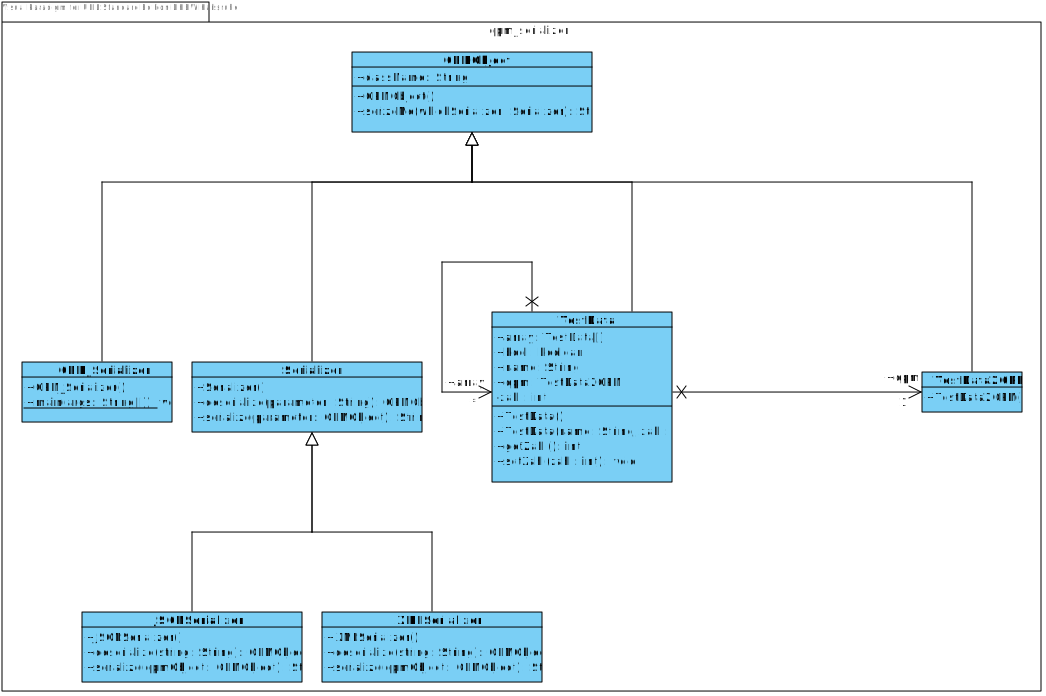
\includegraphics[width=16cm]{Bilder/Erstes_EKD}
\label{Klassendiagramm der Serialisierung}
\caption{Klassendiagramm der Serialisierung} 
\end{figure}

\subsection{JSON-Schema Erstellung aus einer Klasse}\label{JSON-Schema}
\"Ahnlich bei auch bei XML gibt es in JSON ein Datenformat, welches die zu erwartende Form des Streams vorgibt.
Wie auch in XSD wird das Schema in der eigenen Norm als konformes Dokument erstellt. \cite{JSON_Schema}

Ein Beispiel f\"ur ein JSON-Schema wird hier Anhand des JSON-Dokuments in Kapitel \ref{Der Aufbau von JSON} dargestellt.
Das JSON-Schema besteht aus einem Objekt, welches die jeweiligen Namen und Werte der Attribute einer Instanz enth\"alt.

Somit steht am Anfang eines JSON-Schemas immer der Bezeichner \texttt{type} mit dem entsprechenden Wert, n\"amlich \texttt{object}.
Unter dem Schl\"ussel \texttt{properties} sind wiederum als inneres Objekt die Attribute mit ihren m\"oglichen auspr\"agungen aufgelistet. 

Am Anfang einer Propertie steht der Attributname \texttt{"}\texttt{String"}, wie im Beispiel unten.
Gefolgt wird dieser Name von einem Objekt, welches die genauen Eigenschaften des Attributs beschreibt.
Im Beispiel wird einfach nur der Typ des Attributs bezeichnet, jedoch ist auch m\"oglich weitere Einschr\"ankungen \"uber Annotationen zu machen. Mit dessen Hilfe k\"onnte man zum Beispiel einen Wertebereich f\"ur Zahlen angeben.

Um die XML-Annotationen von JAXB bei der Schemaerzeugung zu nutzen muss wieder ein \texttt{AnnotationInspector} verwendet werden.

Die Einschr\"ankungen und Beschreibungen der Attribute werden dem Serializer mit Hilfe der Annotationen \"ubergeben, welche Java-Methoden-Namen enthalen . Das setzen der Beschreibungen geschieht \"uber Java-Methoden welche zur Laufzeit vom Serializer aufgerufen werden.

Auf die Erkl\"arung der einzelnen Annotationen von JAXB wird an dieser stelle verzichtet, da dieses Thema zu Umfangreich ist um es in dieser Arbeit abzuhandeln. 

\lstinputlisting{Code/JSON_Schema.json}

\subsection{JSON-Schema mit Hilfe von Jackson erstellen}
Seit der Jackson Version 2.2 wurde das Modul zur Erstellung eines JSON-Schemas aus dem Modul "`jackson-databind"' ausgegliedert und ein eigenes Modul mit erweitertem Funktionsumfang eingef\"uhrt. 

F\"ur die Erstellung eines JSON-Schemas wird somit das Zusatzmodul \\"`jackson-module-jsonSchema"' ben\"otigt. Um unn\"otige Fehlerquellen zu vermeiden wurde auch dieses Modul in der Version 2.4.1 verwendet, auch wenn es zum Erstellungsdatum schon eine neuere Version gab. Somit sind alle Module von der selben Version und Fehler durch Versionsunterschiede sind ausgeschlossen.

Wie schon in fr\"uheren Beispielen gezeigt wird zu erst wieder ein \texttt{ObjectMapper} erstellt. Hierbei kann eine JsonMappingException auftreten, welche entweder weiter gewurfen werden kann oder dirket behandelt wird.
Des weiteren wird f\"ur die Schemaerzeugung noch ein \\\texttt{SchemaFactoryWrapper} erstellt, welcher das Schema erstellt.
Der Schema-Wrapper kann unter umst\"anden die JsonProcessingException werfen.

Dem Wrapper wird nun \"uber den n\"achsten Methodenaufruf auf den Mapper und die entsprechend zu Mappende Instanz angesetzt. Dies geschieht \"uber die Methode \\\texttt{acceptJsonFormatVisitor}.

Mittels der Methode \texttt{finalSchema} wird das Schema der Instanz als \texttt{JsonSchema} erstellt.

\"Uber den \texttt{return}-Wert wird das \texttt{JsonSchema} als String \"ubergeben.

Im Codebeispiel unten wird dieser Zusammenhang noch einmal verdeutlicht.

\lstinputlisting{Code/generateSchema.java}

\subsection{Auff\"alligkeiten beim Testen}
Beim Serialisieren und Deserialisieren sollen Attribute in JSON-Dokumenten gespeichert werden. Hief\"ur ben\"otigen alle Klassen einen Standard-Konstruktor damit der Serializer diesen Aufrufen kann. 

Des weiteren ben\"otigt der Serializer f\"ur alle nicht \texttt{public} Attribute Getter- und Settermethoden um Zugriff auf diese Attribute zu erhalten. Denn der Serializer darf durch Java-Richtlinien nur auf \texttt{public} Attribute ohne Getter- und Settermethoden zugreifen.

Um eine Serialisierung von allen Klassen zu gew\"arleisten muss eventuell das OPM-Modell angepasst werden.
Da alle Klassen sich an die OPM-Regeln halten, ist somit gew\"ahrleistet das alle ankommenden Instanzen serialisiert oder deserialisiert werden k\"onnen.

In ersten Tests mit dem JSONSerializer wurde die Funktionsf\"ahigkeit bewiesen. Jedoch ist der derzeitige Stand des Serialisierers noch nicht in der Lage verschiedene Klassen zu deserialisieren. Bisher ist der Klassenname fest vorgebeben.

Im Projekt aber sollen unterschiedlichste Klassen deserialisiert werden k\"onnen. Das wirft die Frage auf wie Festgestellt wird, um welche Klasse es sich bei der Instanz handelt. Dieser Punkt wird nun in den folgenden Kapiteln ausf\"uhlich erl\"autert.

\subsubsection{Auff\"alligkeiten beim erstellen des JSON-Schemas}
Nach einigen Tests wurde festgestellt, das Jackson f\"ur alle Zahlen immer \texttt{integer} im Schema angibt, obwohl JSON auch \texttt{double} oder \texttt{float} kennt. Egal ob es sich in der Klasse um \texttt{float, double} oder  \texttt{integer} handelt. Warum dies im Schema nicht Ordnungsgem\"a\ss{} \"ubernommen wird, konnte nach einiger recherche nicht herausgefunden werden.
\newpage
\section{Der SMD-Assistent im GDS-System}
Die \ac{SMD} enthalten alle wichtigen Informationen um die Strucktur einer Klasse zu beschreiben. Diese Klasseninformationen sollen sp\"ater von einem SMD-Assistent verwaltet werden.

In einer MySQL-Datenbank k\"onnen alle Klasseninformationen abgelegt werden. Zu diesen Informationen z\"ahlen zum Beispiel der Klassenname, Attribute mit Modifier, Methoden mit Modifier Parametern und R\"uckgabetyp. 

Da es sich bei den \ac{SMD} um reine Metadaten handelt, werden keine Methodenr\"umpfe in die \ac{SMD}-Datenbank aufgenommen.

Der Nutzer des \ac{GDS}-Systems gibt \"uber den \ac{UDDE}, also das User Interface, seine Klassen und \ac{AMD} in das System.
Unter \ac{AMD} werden die zu seinen Klassen passenden Instanzen bezeichnet, welche der User der Anwendung zum Speichern \"ubergibt.
Des weiteren legt der \ac{UDDE} die generierten "`strukturellen Metadaten"' in einer Datenbank ab, welche sp\"ater vom SMD-Assistent ausgelesen werden k\"onnen.

Der SMD-Assistent ist also f\"ur das Umwandeln von Klassen in \ac{SMD}s verantwortlich. Nach dem erstellen der \ac{SMD}s werden diese zur Aufbewahrung vom Assistenten dem \ac{GDS} \"ubergeben, welcher die Ablage der Daten in einer Datenbank verwaltet.

Die \ac{SMD}s werden von der Anwendung an verschiedenen Stellen ben\"otigt. Der \ac{CG} wandelt die \ac{SMD}s wieder in Java-Klassen, welche OPM-Konform erzeugt werden. Eine genaue Spezifikation f\"ur den Klassengenerator ist im Kapitel \ref{CG} zu finden.
Die generierten Datenstr\"ome k\"onnwn dann ebenfalls vom \ac{GDS} in einer Datenbank gespeichert werden.

Der \ac{IG} erstellt aus den vom SMD-Assistenten gelieferten \ac{SMD}s Schemen f\"ur JSON und XML. Eine Funktion zur Erstellung des JSON-Schemas aus einer Klasse wird in Kapitel \ref{JSON-Schema} beschreiben.
Auch das entsprechnde Klassenschema soll vom \ac{GDS} in einer Datenbank abgelegt werden.

Der beschriebene Zusammenhang der Komponenten des \ac{GDS} ist im Bild unten noch einmal verdeutlicht.

\begin{figure}[!ht]
\centering
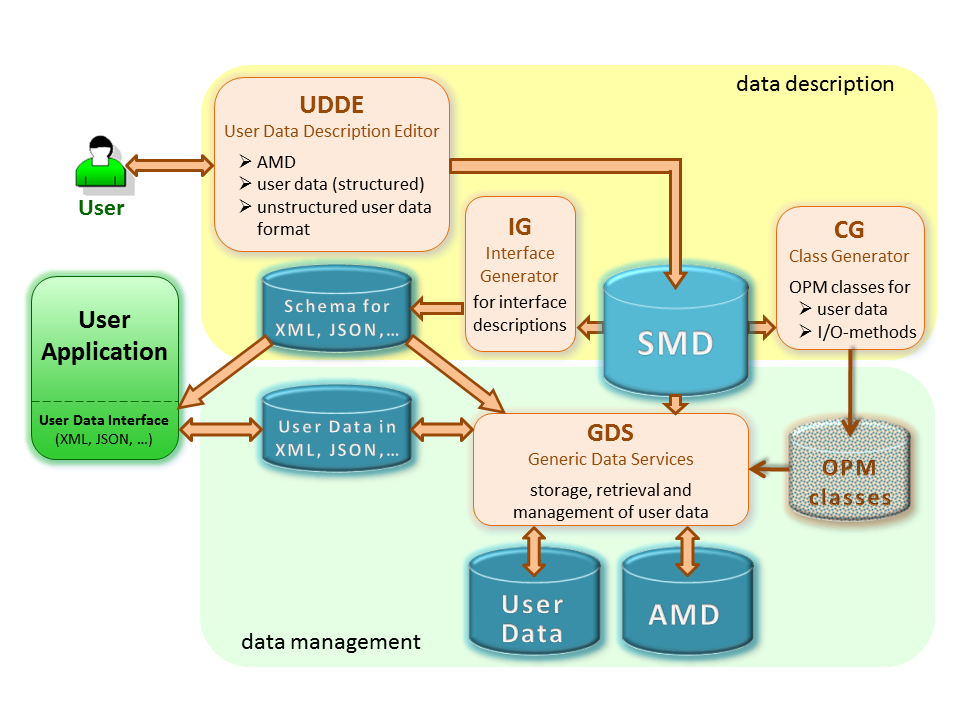
\includegraphics[width=13.5cm]{Bilder/UebersichtGDS}
\title{GDS \"Ubersicht}
\caption{GDS \"Ubersicht}
\centering
\end{figure}

\FloatBarrier

\subsection{Spezifikation des SMD-Assistent}
Im Verlauf der Arbeit wurde zunehmend klar, das die Spezifikation des SMD-Assistent n\"otig wird. Da er, wie im Schaubild oben zu erkennen, zentraler Bestandteil des Projektes ist.
Der SMD-Assistent wurde im Projekt \"offter diskutiert und soll an dieser stelle einmal genauer erleutert werden.

\subsubsection{Funktionen des SMD-Assistent}
Der SMD-Assistent soll die "`strukturellen Metadaten"' aus der Datenbank laden und diese an das \ac{GDS}, den \ac{IG} oder den \ac{CG} weiterreichen. 

Zu einer ObjectID, einer InstanzID oder einem Klassennamen m\"ussen die passenden Metadaten aus der Datenbank geladen werden.
Die geladenen Daten werden in einer Instanz der Klasse \texttt{ClassDecr} zusammengafasst und mittels dieser Instanz \"ubergeben.

Eine Instanz der Klasse \texttt{ClassDecr} enth\"alt mittels der Klassen \texttt{MethodDescr} und \texttt{AttrDecr} alle n\"otigen Informationen um eine Klasse rekonstruieren zu k\"onnen.

\texttt{MethodDescr} enth\"alt eine Methode der Klasse, mit einer Liste von allen Parametern und deren Typen.
Die Klasse \texttt{AttrDecr} hingegen h\"alt jeweils ein Attribut mit dessen Informationen wie zum Beispiel Type und Modifier. \cite{Zil14}

Der Zusammenhang ist im Klassendiagramm der SMD-Klassen noch einmal dargestellt. Im Bild ist aus Gr\"unden der \"Ubersichtlichkeit nicht der gesamte OPM-Klassenbaum abgebildet, sondern lediglich die f\"ur den SMD-Assistent wichtige Klassen sind aufgef\"uhrt.

Einmal aus der Datenbank geladene \ac{SMD}s soll der SMD-Assistent zwischenspeichern, um beim erneuten Abfragen schneller reagieren zu k\"onnen. 

Damit es nicht zu einem Arbeitsspeicher \"uberlauf kommt, muss der SMD-Assistent genau wie alle anderen Assistenten auch eine M\"oglichkeit besitzen den Zwischenspeicher zu verkleinern. Dies soll \"uber einen m\"oglichst effizienten Scheduling-Algorithmus geschehen, welcher Implementiert und auf Effizienz gepr\"uft werden muss.

Hier kommt ein weiterer Assistent zum Einsatz, und zwar der Speicher-Assistent, welcher bei geringem Arbeitsspeicher einen Befehl an alle Assistenten schickt, damit diese ihren Speicherbedarf reduzieren.

\begin{figure}[!ht]
\centering
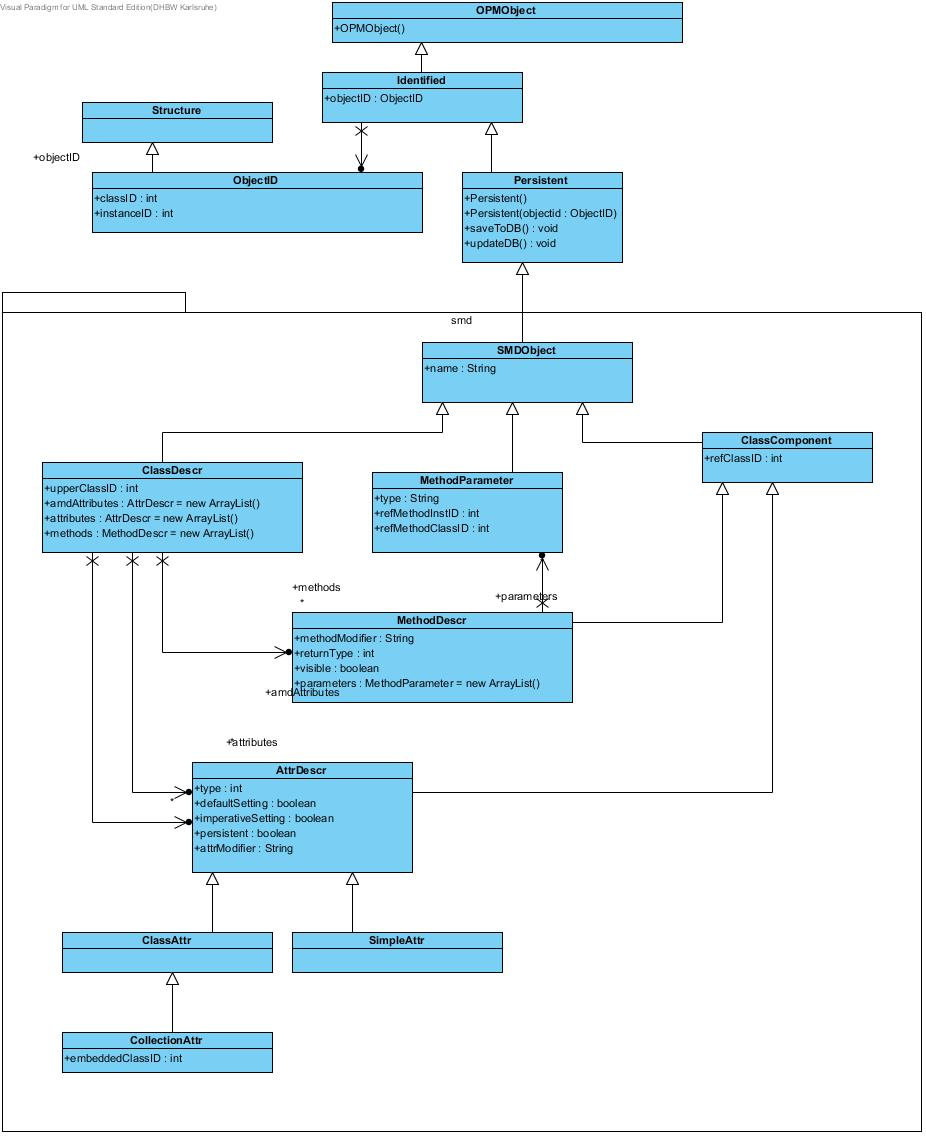
\includegraphics[width=13cm]{Bilder/SMD_Klassen}
\title{Klassendiagramm der SMD-Klassen}
\caption{Klassendiagramm der SMD-Klassen}
\centering
\end{figure}

\subsubsection{Der SMD-Assistent unter Java}
Unter Java kann die Arbeitsweise des SMD-Assistent deutlich vereinfacht werden, da hier die \ac{SMD}s nur bei explizitem verlangen geliefert werden m\"ussen, denn Java verwendet mit den \textit{.class}-Files eigene Metadaten \"uber die eine Verarbeitung unter Java einfacher Umgesetzt werden kann. 
Der SMD-Assistent sollte unter Java also in der Lage sein direkt \textit{.class}-Files zu liefern.

\subsection{Der Klassengenerator} \label{CG}
Der Klassengenerator ist ein Modul des \ac{GDS}, welcher aus den vom SMD-Assistenten gegebenen strukturellen Metadaten wieder Klassen generiert. Es gibt eine abstrakte Klasse \texttt{ClassGenerator} welche abstrakte Methoden zur Verf\"ugung stellt. 

F\"ur jede Programmiersprache, soll nun ein Klassengenerator von der abstrakten Oberklasse abgeleitet werden. Die Programmiersprachen spezifischen Klassengeneratoren sind dann in der Lage, f\"ur ihre Programmiersprache aus den \ac{SMD}s Klassen zu generieren.

Da die Serialisierer wie Jackson und JAXB f\"ur Attribute die nicht \texttt{public} sind Getter- und Setter-Methoden ben\"otigen muss der Klassengenerator diese erzeugen, auch wenn diese Nicht in den \ac{SMD}s auftauchen. Des weiteren muss er diese Methoden auch nach standard implementieren. Dies bedeutet, das in Setter-Methoden die Attribute gesetzt und in Getter-Methoden die Attribute  gelesen werden m\"ussen.

Au\ss{}erdem ben\"otigen die Serialisierer auch Standardkonstruktoren um ein leeres Element zu erstellen, welches im Laufe der Deserialisierung gef\"ullt werden kann.

Um die Serialisierer steuern zu k\"onnen sind gegebenenfalls Annotationen an den Klassen Notwendig, welche ebenfalls vom \texttt{ClassGenerator} angebracht werden m\"ussen.




\newpage
\section{Test des JSON-Serialisierers}
Im Verlauf dieses Kapitels wird die ben\"otigte Arbeitszeit zum Serialisieren und Deserialisieren, sowie das Verhalten von Jackson genauer untersucht und eine Auswertung dieser Tests vorgenommen.

\subsection{Testaufbau}
Im Test wird der Quellcode, wie im Verlauf der Arbeit beschrieben, eingesetzt, um das Verhalten der \ac{JSON}-Bilbliothek genauer zu beurteilen.
Hierf\"ur wurden die beiden vorl\"aufigen Testklassen wurden durch sinnvolle Testklassen ersetzt .

In den folgenden Unterkapiteln zum Testaufbau ist immer nur von Serialisierung die Rede, was aus \"Ubersichtlichkeitsgr\"unden getan wurde. Gemeint ist jedoch nicht nur die Serialisierung, sondern auch die Deserialisierung.

\subsection{Testaufbau Software}
Der Test wird mit speziell f\"ur Testzwecke geschriebene Klassen durchgef\"uhrt, wobei es sich um f\"unf Testklassen handelt.

Die erste Klasse enth\"alt genau einen \texttt{short}-Wert als Attribut zur Serialisierung. Mit Hilfe dieser Klasse soll, unter Beachtung der anderen Tests, herausgefunden werden, wie lange der Anlauf und das Ausf\"uhren einer Serialisierung ben\"otigt. Diese Aussage ist m\"oglich, da abgesehen von zwei Byte keine weiteren Daten der Klasse serialisiert werden und somit sollte die Bearbeitung eines Attributs keine Auswirkung haben.

Eine Klasse, welche genau ein Gibibyte ($2^{30}$ = 1 073 741 824 Byte) an Daten beinhaltet, soll etwas \"uber die Zeit f\"ur die Serialisierung von einem Element aussagen, da hier die Zeit f\"ur das Anlaufen des Serialisieres vernachl\"assigt werden kann.
Um die Datenmenge zu erreichen wird, eine Klasse mit 536 870 912 \texttt{short}-Werten in einem Array erzeugt, denn jeder \texttt{short}-Wert ist 2 Byte gro\ss{}, wodurch sich die genaue Gr\"o\ss{}e von einem Gibibyte ergibt. Die \texttt{short}-Werte werden im Konstruktor bei Erstellung der Klasse zuf\"allig erzeugt.

Die dritte Testklasse enth\"alt von jedem m\"oglichen "`Standard-Datentyp"' genau ein Attribut mit einem Wert. Sie dient haupts\"achlich als Vergleichspunkt zu den beiden noch fehlenden Klassen, aber auch um zu beweisen, dass jeder Datentyp serialisiert werden kann.

Eine weitere Klasse ist genau wie die dritte beschriebene Vergleichsklasse aufgebaut, jedoch mit dem Unterschied, dass diese ein weiteres Attribut besitzt. Bei dem neuen Attribut, handelt es sich um ein Klassenattribut, welches der dritten, beschriebenen, Klasse entspricht.
Gepr\"uft werden soll nun, ob die Serialisierung \"ahnlich lange wie bei der dritten Klasse dauert. Sollte das der Fall sein beinhaltet der eingesetzte Serialisierer einen Cache, bzw. arbeitet vorausschauend.

Bei der letzten zu testenden Klasse handelt es sich um eine rekursive Version der dritten Klasse, wobei zwei Rekursionsstufen gemacht werden. Hier soll gepr\"uft werden, wie der Serialisierer mit Rekursion umgeht, und welche Zeit er hierf\"ur beansprucht.

\newpage
\subsection{Testaufbau Hardware}
Die Tests wurden auf einem Arbeitsplatzrechner mit Kubuntu 12.04.2 Linux 3.2.0.58-generic x86-64 durchgef\"uhrt.

Die Hardwaredaten des Rechners waren folgende:
\begin{itemize}
 \item CPU: 2x Intel Xeon 5148 mit 2,33 GHz
 \item RAM: 8GB DDR-2 667 MHz (Zugriffszeit 1,5 ns)
 \item Chipsatz: Intel 5000 Series Chipset
 \item Festplatte: Seagate ST31000528AS (1 TB) davon 16 GB Swap
\end{itemize}
Zur Festplatte sollte noch gesagt sein, das sich das Betriebssystem, Swap und Datenpartition jeweils auf getrennten Partitionen befinden, jedoch physisch auf einer Festplatte sind.

Bei allen Tests wurde darauf geachtet, dass der Swap nicht benutzt wird, um Verzerrungen der Messzeit zu verhindern.

\subsection{Testdurchf\"uhrung}
Die Testdurchf\"uhrung wurde zuerst zusammenh\"angend ausgef\"uhrt, dass hei\ss{}t, alle Tests wurden automatisiert vom Programm ausgef\"uhrt. Jedoch wurden sehr fr\"uh Effekte verschiedener Caching-Mechanismen festgestellt, was eine genaue Messung der Tests auf diese Art nicht m\"oglich macht. 

Zum einen werden bei der automatischen Testausf\"uhrung Hardware-Caches verwendet, zum anderen ist der JIT-Compiler in der Lage, diesen Testablauf weiter zu optimieren. Um dies zu verhindern, wurde wie folgt vorgegangen.

Es wurde somit entschieden, jeden Test einzeln durchzuf\"uhren und ihn jeweils dreimal zu wiederholen, wenn keine extremen Schwankungen auftreten. Sollte das der Fall sein muss ein Test \"ofters wiederholt werden, bis die Testzeit eindeutig ist.

\subsubsection{Auff\"alligkeiten bei Testbeginn}
Die gr\"o\ss{}te Klasse mit einem Gibibyte Daten bereitetete Probleme. 
Jackson ist nicht in der Lage, so viele Elemente in einer Instanz zu serialisieren.

Dies liegt daran, dass bei einer solch gro\ss{}en Datenmenge extrem gro\ss{}e Strings entstehen, welche die \texttt{StringBuffer}-Klasse, die intern in Jackson verwendet wird, nicht verarbeiten kann, da diese auf Arrays bassiert, welche die Gr\"o\ss{}e beschr\"anken.

Da dieser Effekt auch bei f\"unfhundert Mebibyte auftrat, wurde entschieden, die gro\ss{}e Klasse auf zweihundertf\"unfzig Mebibyte zu beschr\"anken. Daraus resultiert, dass sich nur noch 134 217 728 \texttt{short}-Werte im Array befinden. Was eine Datengr\"o\ss{}e von 256 Mebibyte darstellt.

Dieser Effekt, zeigt sich jedoch nur bei der \texttt{jre-1.7.0.60 Open-JDK}. Das Java Runtime Environment der Firma Oracle funktioniert genau wie die \texttt{jre-1.7.0.45 Open-JDK-Bibliothek} bis zu einer Klassengr\"o\ss{}e von 512 Gibibyte fehlerfrei.

\subsection{Testergebnisse}
Die folgenden Testergebnisse wurden wie oben beschrieben ermittelt, wobei die Endzeit in Millisekunden des Vorgangs von der Startzeit in Millisekunden angezogen wurde.

Das Serialisieren einer Klasse mit einem \texttt{short}-Wert dauerte bei drei Durchg\"angen 338, 335 und 337 Millisekunden. Die Deserialisierung betrug im Gegensatz dazu wesentlich weniger Zeit, n\"amlich 40, 40 und 41 Millisekunden. 

Die Klasse mit allen m\"oglichen Datentypen ben\"otigte f\"ur die Serialisierung  355, 344 und 346 Millisekunden. Das Deserialisieren ben\"otigte kaum mehr Zeit als bei nur einem Wert und zwar 46, 46 und 50 Milisekunden.

Ein Klassenattribut in einer Klasse ben\"otigte f\"ur das Serialisieren 355, 341 und 342 Millisekunden. Die Deserialisierung dauerte 49, 50 und 49 Millisekunden

Derselbe Dateninhalt, jedoch rekursiv aufgerufen, brauchte zum Serialisieren 343, 339 und 347 Millisekunden. Beim Deserialisieren ergaben sich 47, 47 und 48 Millisekunden.

Das Serialisieren der gro\ss{}en Klasse ben\"otigte 10632, 10751 und 10521 Millisekunden. Zum Deserialisieren wurde eine Zeit von 17012, 16836 und 17127 Millisekunden ben\"otigt.

\subsection{Auswertung der Testergebnisse}
Aus der Serialisierung der gro\ss{}en Klasse l\"asst sich sehr gut entnehmen, dass die Serialisierung eines einzelnen Elements quasi keine Zeit in Anspruch nimmt, denn die Zeit f\"ur ein Element liegt bei $7,67111*10^{-5}$ Millisekunden.

\"Uber Jackson kann also ausgesagt werden, dass das Starten des Serialisierungsprozesses in etwa 336 Millisekunden dauert, da das Serialisieren einer Klasse mit einem Attribut im Mittel diese Zeit ben\"otigt und somit die Serialisierung dieses Attributs vernachl\"assigt werden kann, da es quasi keine Zeit in Anspruch nimmt, wie die Serialisierung der gro\ss{}en Klasse gezeigt hat.

Auch durch die folgenden Ergebnisse ist diese Aussage  m\"oglich. Da auch eine Klasse mit mehreren Elementen (Klasse mit jeweils einem Attribut von jedem Datentyp) mit 348,3 Millisekunden eine \"ahnlich lange Zeit ben\"otigt, wie die Klasse mit einem Element.

Auch das Serialisieren und Deserialisieren von Klassenattributen und Rekursion wird anscheinend sehr gut optimiert, da sich im direkten Vergleich zu der einfachen Klassen keine wesentlichen zeitlichen Unterschiede ergeben.

Hier kommt auch gut zur Geltung, wie stark Java optimieren kann, denn bei der kleinen Klasse wird f\"ur jedes Element im Schnitt eine Millisekunde ben\"otigt, was im krassen Gegensatz zu 0,000071 Millisekunden steht. Diese extreme Beschleunigung wird zum einen durch Caching-Mechanismen, zum anderen auch vom JIT-Compiler und der daraus folgenden Parallelisierung hervorgerufen. 

Welche Mechanismen wo genau ansetzten und wie sie im speziellen angewendet werden, wurde im Rahmen dieser Arbeit nicht untersucht.

Bei langen Strings dauert das Deserialisieren pl\"otzlich l\"anger als das Serialisieren, was daher r\"uhrt, dass bei der Klassennamensuche der komplette String durchlaufen werden muss.

\subsection{Zusammenfassung der Testergebnisse}
Obwohl bei der Deserialisierung der ankommende String erst auf die zugeh\"orige Klasse gepr\"uft werden muss, ist die Deserialisierung deutlich schneller erledigt als eine Serialisierung. Dies l\"asst darauf schlie\ss{}en, dass es einfacher und schneller geht, Objekte zu bauen als diese zu speichern.

Die Serialisierung mit Jackson ist zum einen schnell, zum anderen aber auch sehr Arbeitsspeicher intensiv. Beim Testen konnte beobachtet werden, wie beim Serialisieren der allokierte Arbeitsspeicher sprunghaft ansteigt. Es zeigte sich, dass mindestens vier mal so viel RAM ben\"otigt wird, wie die zu serialisierende Datei gro\ss{} ist. 








% % \newpage
% \include{Lastenheft}
% \newpage
% % \include{Pflichtenheft}
% % \newpage
% \include{Software_Analyse}
% \newpage
% \include{Datenbank_Analyse}
% \newpage
% \include{Implementierung}
% \newpage
% \include{weiteres_vorgehen}
% \newpage
% \include{Intialisierung_des_Ladevorgangs_aus_der_Datenbank}
% \include{Initialisieren_der_ICubeDataSource}
% \include{Fazit}
% \include{Anhang}

\end{spacing}

%Einf�gen Inhaltsverzeichnis


\newpage
\section{Abk�rzungsverzeichnis}
\begin{acronym}
 \acro{KIT}{\emph{Karlsruher Instituts f�r Technologie}}
 \acro{GDS}{\emph{generisches Managementsystem f\"ur Energiedaten}}
 \acro{LSDF}{\emph{Large Scale Data Facility}}
 \acro{OPM}{\emph{objektorientierten Programmiermodell}}
 \acro{SMD}{\emph{strukturelle Metadaten}}
 \acro{JSON}{\emph{JavaScript Object Notation}}
 \acro{HALO}{\emph{High Altitude and Long Range Research Aircraft}}
 \acro{IAI}{\emph{Institut f�r Angewandte Informatik}}
 \acro{JAXB}{\emph{Java Architecture for XML Binding}}
\end{acronym}
% Abk�rzungsverzeichnis
\newpage
\bibliographystyle{alphadin}
% verzeichnis im DIN format
\bibliography{Quellen}
\end{document}
